% !TEX root = main.tex
\IfFileExists{elsarticle.cls}{
  \documentclass[preprint,12pt]{elsarticle}
  \newif\ifelsevierclass\elsevierclasstrue
}{
  \documentclass[12pt]{article}
  \newif\ifelsevierclass\elsevierclassfalse
}

\usepackage[utf8]{inputenc}
\usepackage[T1]{fontenc}
\usepackage{lmodern}
\usepackage{amsmath,amssymb}
\usepackage{booktabs}
\usepackage{graphicx}
\usepackage{array}
\usepackage{xcolor}
\usepackage{microtype}
\usepackage{hyperref}
\hypersetup{colorlinks=true,linkcolor=black,citecolor=black,urlcolor=blue}
\graphicspath{{generated/figures/}}
\emergencystretch=3em

\newcommand{\ReT}{\mathrm{ReT}}
\newcommand{\HOL}{H_{\mathrm{OL}}}
\newcommand{\DeltaN}{\Delta_{N}}

\begin{document}

\ifelsevierclass
\begin{frontmatter}
\title{When Feedback Beats Every Static Policy but Not Structured Control: Exact Benchmarking of Recurrent RL in a Supply-Chain DES}
\author{Anonymous for review}
\begin{abstract}
Reinforcement learning (RL) can outperform a short list of fixed supply-chain policies without demonstrating that a neural controller is necessary. We separate the value of feedback from a specifically neural premium in a thesis-grounded, researcher-defined multiproduct extension of a discrete-event military food-supply-chain model. The weekly decision allocates three production batches between two non-fungible products over eight weeks, yielding an exactly enumerable frontier of $4^8=65{,}536$ open-loop calendars. The primary resilience functional reproduces 47,546 cells of the source Excel workbooks with zero discrepancy when supplied the source ledger snapshots. Ten frozen RecurrentPPO policies were prospectively evaluated on 256 new common-random-number tapes in each of three demand-regime cells. RecurrentPPO exceeded the best calendar in the complete static frontier by 0.07255--0.11724 in mean Excel ReT; simultaneous lower confidence bounds were 0.06233--0.10614, and all ten optimizer seeds were positive in every cell. Against the best reselected structured controller, however, the differences were -0.00159 to -0.00041 and all simultaneous intervals lay within the prespecified $\pm0.01$ equivalence region. The frozen worst-product-fill non-inferiority condition was not established. Thus feedback has robust value in this contract, but neural superiority and deployment safety do not. The study contributes an exact static benchmark, a comparator-rights protocol, and a reproducible claim ladder for deciding when learned control is warranted in industrial simulation.
\end{abstract}
\begin{keyword}
supply chain resilience \sep reinforcement learning \sep discrete-event simulation \sep exact benchmark \sep structured feedback control \sep reproducibility
\end{keyword}
\end{frontmatter}
\else
\title{When Feedback Beats Every Static Policy but Not Structured Control: Exact Benchmarking of Recurrent RL in a Supply-Chain DES}
\author{Anonymous for review}
\date{}
\maketitle
\begin{abstract}
Reinforcement learning (RL) can outperform a short list of fixed supply-chain policies without demonstrating that a neural controller is necessary. We separate the value of feedback from a specifically neural premium in a thesis-grounded, researcher-defined multiproduct extension of a discrete-event military food-supply-chain model. The weekly decision allocates three production batches between two non-fungible products over eight weeks, yielding an exactly enumerable frontier of $4^8=65{,}536$ open-loop calendars. The primary resilience functional reproduces 47,546 cells of the source Excel workbooks with zero discrepancy when supplied the source ledger snapshots. Ten frozen RecurrentPPO policies were prospectively evaluated on 256 new common-random-number tapes in each of three demand-regime cells. RecurrentPPO exceeded the best calendar in the complete static frontier by 0.07255--0.11724 in mean Excel ReT; simultaneous lower confidence bounds were 0.06233--0.10614, and all ten optimizer seeds were positive in every cell. Against the best reselected structured controller, however, the differences were -0.00159 to -0.00041 and all simultaneous intervals lay within the prespecified $\pm0.01$ equivalence region. The frozen worst-product-fill non-inferiority condition was not established. Thus feedback has robust value in this contract, but neural superiority and deployment safety do not.
\end{abstract}
\fi

\section{Introduction}

Discrete-event simulation (DES) is widely used to examine supply-chain disruption and recovery, but a conventional simulation commonly evaluates policies chosen before the run. This open-loop use is appropriate for comparing doctrines, yet it cannot by itself represent an organization that observes an evolving system and revises decisions. Garrido and colleagues identify this separation between simulated experience and subsequent decision making as a central limitation of supply-chain-resilience simulation and propose artificial intelligence as a bridge that closes the decision loop \cite{garrido2024iccl}. The open methodological question is not merely whether a learned policy can beat a fixed baseline. It is whether the improvement comes from feedback that any competent controller could exploit, or from a residual capability that requires a neural learner.

That distinction matters because RL studies in inventory and supply-chain control often compare against a small set of heuristics, while strong problem-specific controllers can absorb much of the available state-contingent value \cite{boute2022,gijsbrechts2022,powell2022}. A learner that beats a weak static baseline may have rediscovered a better calendar. Conversely, practical outcome equivalence does not imply a computational advantage for either controller. Benchmark design therefore determines the scientific meaning of an ``RL gain.''

We study this question in a full DES reconstructed from the 13-operation military food-supply-chain model of Garrido-Rios \cite{garrido2017}. We disclose a researcher-defined extension with two non-fungible product classes sharing production capacity. Each week the controller allocates three batch slots between the products. Eight weekly decisions produce exactly 65,536 open-loop calendars, small enough to enumerate completely but rich enough for changing demand regimes to make feedback useful. The primary outcome is the source Excel ReT functional. We reproduce its formula exactly and preserve its workbook-visible population semantics rather than silently replacing it with a more convenient objective.

Our research question is:

\begin{quote}
When a recurrent policy exceeds an exhaustive open-loop frontier, does the gain identify the value of feedback, a specifically neural premium over structured control, and product-level service safety?
\end{quote}

The answer is deliberately decomposed. RecurrentPPO prospectively beats every calendar in the exact static frontier in all three evaluation cells. It does not beat the strongest structured controller; instead, it satisfies a prespecified practical-equivalence test. Product-level non-inferiority is not established. This is not a failed positive claim repackaged after the fact. The learner, comparator family, equivalence margin, guardrails, checkpoints, tapes, and simultaneous inference were frozen before the confirmation data were opened.

The contributions are sixfold. First, we reproduce the source resilience formula and state the population boundary introduced by a workbook-visible ledger. Second, we provide a complete rather than sampled static frontier. Third, we assign explicit information, action, resource, and selection rights to every comparator. Fourth, we separate learned adaptation from a neural premium through simultaneous superiority and equivalence estimands. Fifth, we show that aggregate resilience equivalence does not establish service safety for the worst product. Sixth, we release a hash-addressed pipeline that regenerates all manuscript tables and figures from the frozen adjudication artifacts.

\begin{table}[htbp]
\centering
\small
\caption{Claim ladder and adjudicated boundary.}
\label{tab:claim_ladder}
\begin{tabular}{p{0.16\linewidth}p{0.23\linewidth}p{0.17\linewidth}p{0.32\linewidth}}
\toprule
Level & Question & Status & Evidence boundary \\
\midrule
Metric & Excel ReT reproduced? & Supported & 47,546 workbook rows; zero mismatches \\
Static & Best open-loop frontier known? & Supported & All $4^8=65,536$ calendars evaluated \\
Learned & Feedback beats the exhaustive 65,536-calendar frontier? & Supported & H\_OL LCB95 $>0$ in all three cells; 10/10 seeds positive \\
Neural & RL beats structured control? & Not supported & Delta\_N practically equivalent to zero within $\pm0.01$ \\
Safe & Worst product non-inferior? & Not established & Simultaneous lower bounds cross the frozen $-0.02$ margin \\
\bottomrule
\end{tabular}
\end{table}


\section{Related work and positioning}

Supply-chain resilience concerns the capacity to absorb, respond to, and recover from disruption while maintaining required functions \cite{ponomarov2009understanding,hosseini2019review}. Quantitative research increasingly combines simulation with machine learning, but the evidentiary role of the learner varies: prediction can inform a fixed policy, RL can choose sequential actions, and simulation optimization can search an open-loop design \cite{badakhshan2024,yan2022,rolf2023}. These are not interchangeable forms of adaptation.

Deep RL has produced important results in lost-sales, dual-sourcing, and multi-echelon inventory problems \cite{gijsbrechts2022}. At the same time, the inventory-control literature emphasizes the importance of structured baselines, reward design, and state sufficiency \cite{boute2022}. Our study focuses on an identification problem left implicit by performance-only comparisons: if a neural policy beats every static design but not a structured feedback family with the same deployable information, the evidence supports feedback value without supporting neural necessity.

The distinction also connects to simulation optimization. Selecting the maximum observed response from a large design set can create winner's-curse bias unless the selection and evaluation protocol are separated \cite{boesel2003}. We avoid this in two ways. The static frontier is exhaustive, and its best calendar is selected by mean performance rather than per-tape future knowledge. In inference, the best open-loop and structured comparators are reselected inside every bootstrap resample. The final estimates use new confirmation tapes opened once.

Garrido et al. propose a broader agenda in which simulated experience becomes accumulated organizational learning \cite{garrido2024iccl}. The present study addresses the prerequisite within-campaign question: whether feedback changes outcomes and whether a neural controller contributes beyond structured feedback. It does not test memory retained across campaigns. That is reserved for a separate prospective study and is excluded from the claims here.

\section{Model and decision contract}

\subsection{Thesis-grounded DES and disclosed extension}

The base simulation follows the material and information flow of the 13-operation model in Garrido-Rios \cite{garrido2017}. The Program Q contract adds two non-fungible product labels, $P_C$ and $P_H$, that share the Op5--Op7 production line. This addition is researcher-defined; the paper does not attribute the product labels or their demand process to the original military system.

An episode contains eight weekly decisions. At decision $t$, action $a_t\in\{0,1,2,3\}$ assigns $a_t$ of the next three batches to $P_C$ and the remainder to $P_H$. Production mass, scheduled transport, demand tapes, and decision frequency are identical across policies. Demand follows a latent two-regime process characterized by persistence $\rho$ and dominant-product share $s$. Evaluation uses three cells: $(.75,.90)$, $(.90,.75)$, and $(.90,.90)$. The primary experiment disables the original risk generators. The resulting claim concerns state-dependent product-mix control under demand-regime uncertainty, not active Garrido-native disruptions.

The open-loop space is the Cartesian product of four actions over eight weeks. We evaluate all
\[
4^8=65{,}536
\]
calendars. The best static policy is the calendar with highest mean ReT across the evaluation tapes. Selecting the best calendar separately after seeing each tape would use future information and is not allowed.

\subsection{ReT functional and ledger boundary}

For order $j$, the source workbooks implement
\[
Re_j=
\begin{cases}
AP_j/LT, & \text{risk active and } AP_j>0,\\
0.5/RP_j, & \text{risk active, } AP_j=0,\ RP_j>0,\\
0, & \text{risk active without recovery},\\
1-(B_{t,j}+U_{t,j})/j, & \text{without active risk}.
\end{cases}
\]
We neither clip nor normalize this formula. With the source $B_t/U_t$ snapshots injected, the repository implementation reproduces all 47,546 formula rows in the available workbooks with maximum absolute error zero.

Formula fidelity does not eliminate a population issue. The primary workbook-visible mean contains completed non-lost orders and therefore does not, by itself, penalize every horizon-unresolved order. We keep the official metric unchanged and treat the complete demand ledger as an identification requirement. Lost demand, unresolved orders and quantities, service-loss area, backlog age, product fills, mass conservation, and scheduled resources are reported separately. Scientific interpretation is consequently constrained optimization: maximize official mean ReT among policies satisfying a frozen ledger and service audit, rather than maximize the visible mean without qualification.

\subsection{Comparators}

The open-loop frontier receives no feedback. The structured family receives the same deployable operational history as the learner and includes belief-based and state-rich feedback rules. The selected structured comparator is the family member with maximum mean ReT, with family reselection performed inside each bootstrap resample. RecurrentPPO receives a 21-field causal observation containing product inventory, locked pipeline, backlog summaries and age, in-flight quantity, a fixed-model HMM belief summary, the previous action, and public phase. It never receives the tape identity, true evaluation-cell parameters, latent regime, future demand, oracle calendar, or score-time outcomes.

\begin{table}[htbp]
\centering
\small
\caption{Information and decision rights of the principal comparators.}
\label{tab:comparators}
\begin{tabular}{p{0.18\linewidth}p{0.23\linewidth}p{0.19\linewidth}p{0.28\linewidth}}
\toprule
Comparator & Information & Decision rights & Resource and selection rule \\
\midrule
Open-loop frontier & No episode feedback & Eight weekly mix actions fixed ex ante & All 65,536 calendars; common tapes and scheduled resources \\
Belief-based control & Same deployable operational history; fixed HMM model & Replans weekly over the same four actions & Best frozen structured controller reselected inside bootstrap \\
RecurrentPPO & Same 21-field causal observation; recurrent state & Chooses one of four mix actions weekly & Ten frozen checkpoints; identical physical resources \\
Oracle & Privileged future information & Diagnostic only & Never a deployable comparator or a learned claim \\
\bottomrule
\end{tabular}
\end{table}


\begin{figure}[htbp]
\centering
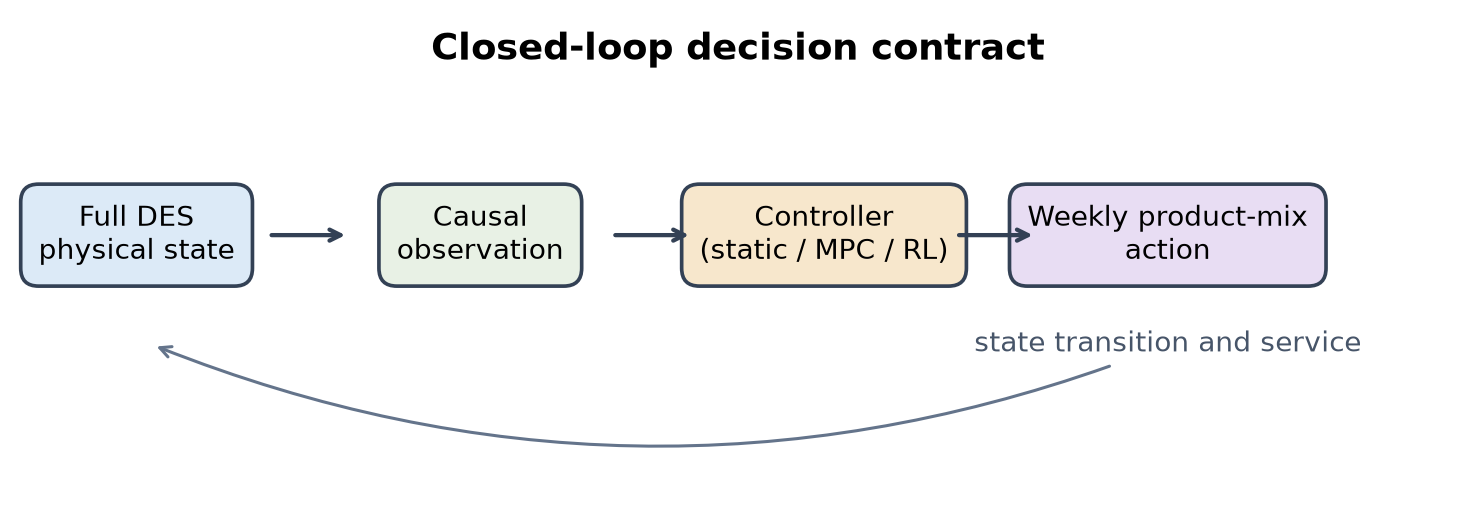
\includegraphics[width=\linewidth]{figure1_closed_loop}
\caption{Decision loop shared by the structured and learned controllers. Only the controller changes; the DES physics, causal observation, action rights, and scheduled resources are common.}
\label{fig:loop}
\end{figure}

\section{Learner and evaluation protocol}

Ten RecurrentPPO policies with optimizer seeds 8101--8110 were trained for 200,192 timesteps each. The policy uses a 64-unit LSTM and a two-layer $[64,64]$ multilayer perceptron. The frozen hyperparameters are learning rate $3\times10^{-4}$, rollout length 512, batch size 64, discount 0.99, GAE 0.95, clipping 0.2, and entropy coefficient 0.01. Reward is zero after decisions one through seven and equals terminal official ReT after the eighth decision. Architecture and checkpoint search were not performed; only the final checkpoint from each seed is evaluated.

Confirmation uses 256 new tapes per cell and common random numbers across policies. The learner checkpoints were frozen by hash before those tapes were opened. The two primary estimands are
\[
\HOL=V(\pi_{\mathrm{RNN}})-V(\pi^*_{\mathrm{OL}}),
\qquad
\DeltaN=V(\pi_{\mathrm{RNN}})-V(\pi^*_{\mathrm{structured}}).
\]
$\HOL$ identifies learned feedback value relative to the complete static frontier. $\DeltaN$ identifies incremental neural value relative to the strongest tested structured controller. The frozen practical-equivalence region for $\DeltaN$ is $[-0.01,0.01]$.

Inference uses a two-way learner-seed/tape studentized max-$t$ bootstrap with 10,000 resamples. Comparators are reselected inside every resample, and intervals are simultaneous across all three cells. The confirmation additionally requires at least 70\% favorable tapes and at least eight of ten positive learner seeds for the learned-adaptation endpoint. The direct audit replayed 21,696 unique full-DES trajectories with no failures and maximum ReT discrepancy below $8\times10^{-16}$.

The feedback audit records complete action trajectories. Each learned checkpoint must generate multiple calendars and vary decisions across weeks. Modal, phase-only, and frequency-matched replacements are then evaluated under the same tapes. These controls distinguish state feedback from a high-performing fixed or phase-coded schedule.

\section{Results}

\subsection{Feedback value and structured-control equivalence}

Figure~\ref{fig:frontier} positions the adaptive controllers relative to the exact calibration frontier. The confirmatory comparison is reported in Table~\ref{tab:confirmation} and Figure~\ref{fig:effects}. RecurrentPPO exceeds the best static calendar by 0.07952, 0.07255, and 0.11724 across the three cells. The simultaneous lower bounds are 0.06608, 0.06233, and 0.10614, respectively. Favorable-tape fractions range from 84.8\% to 95.7\%, and every one of the ten learner seeds has positive $\HOL$ in every cell.

Against structured control, the point estimates are -0.00159, -0.00072, and -0.00041. Their simultaneous bilateral intervals are contained inside $[-0.01,0.01]$. The result supports practical equivalence and rejects the intended interpretation that a positive open-loop contrast, by itself, demonstrates neural superiority.

\begin{figure}[htbp]
\centering
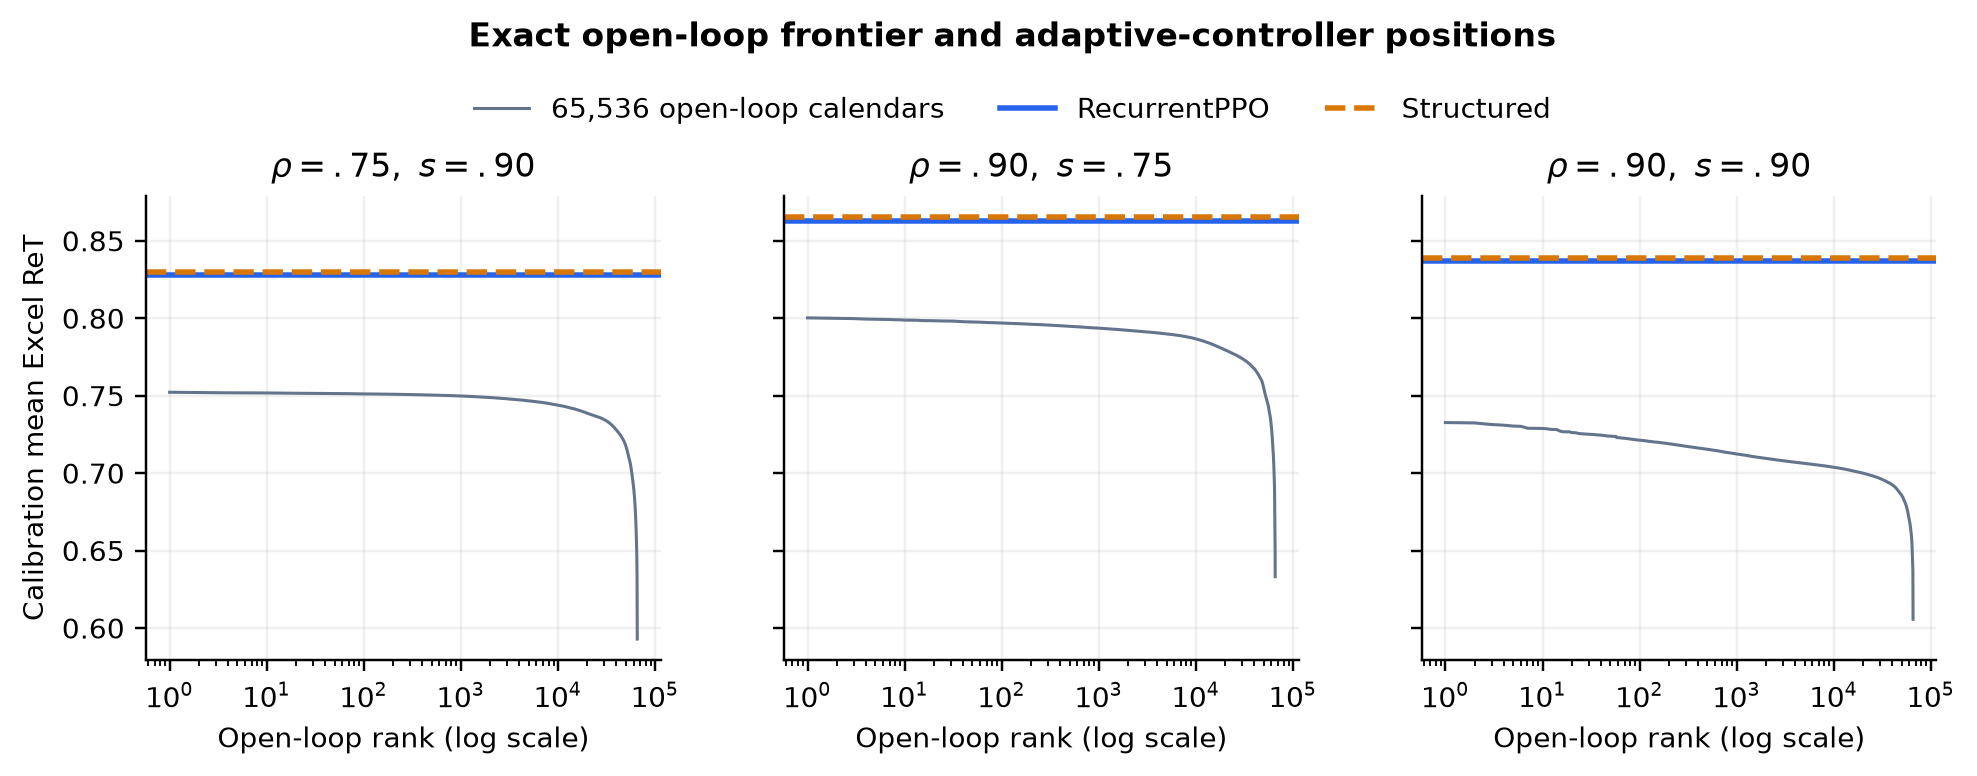
\includegraphics[width=\linewidth]{figure2_static_frontier}
\caption{The complete calibration frontier, with RecurrentPPO and the selected structured controller positioned using calibration contrasts. The frontier is exact; controller lines are descriptive calibration values. Confirmatory inference uses separate tapes in Table~\ref{tab:confirmation}.}
\label{fig:frontier}
\end{figure}

\begin{table}[htbp]
\centering
\small
\caption{Program Q confirmation results on 256 new tapes per cell.}
\label{tab:confirmation}
\resizebox{\linewidth}{!}{%
\begin{tabular}{lrrrrrr}
\toprule
Cell & $H_{OL}$ & LCB95 & $\Delta_N$ & CI95 & Fav. & Seeds \\
\midrule
rho75\_share90 & +0.07952 & +0.06608 & -0.00159 & [-0.00627, +0.00310] & 84.8\% & 10/10 \\
rho90\_share75 & +0.07255 & +0.06233 & -0.00072 & [-0.00552, +0.00408] & 89.8\% & 10/10 \\
rho90\_share90 & +0.11724 & +0.10614 & -0.00041 & [-0.00268, +0.00186] & 95.7\% & 10/10 \\
\bottomrule
\end{tabular}
}
\vspace{2pt}
\parbox{0.96\linewidth}{\footnotesize $H_{OL}$ compares RecurrentPPO with the best of all 65,536 open-loop calendars. $\Delta_N$ compares it with the best structured controller. Intervals are simultaneous two-way learner-seed/tape max-$t$ intervals with comparator reselection.}
\end{table}


\begin{figure}[htbp]
\centering
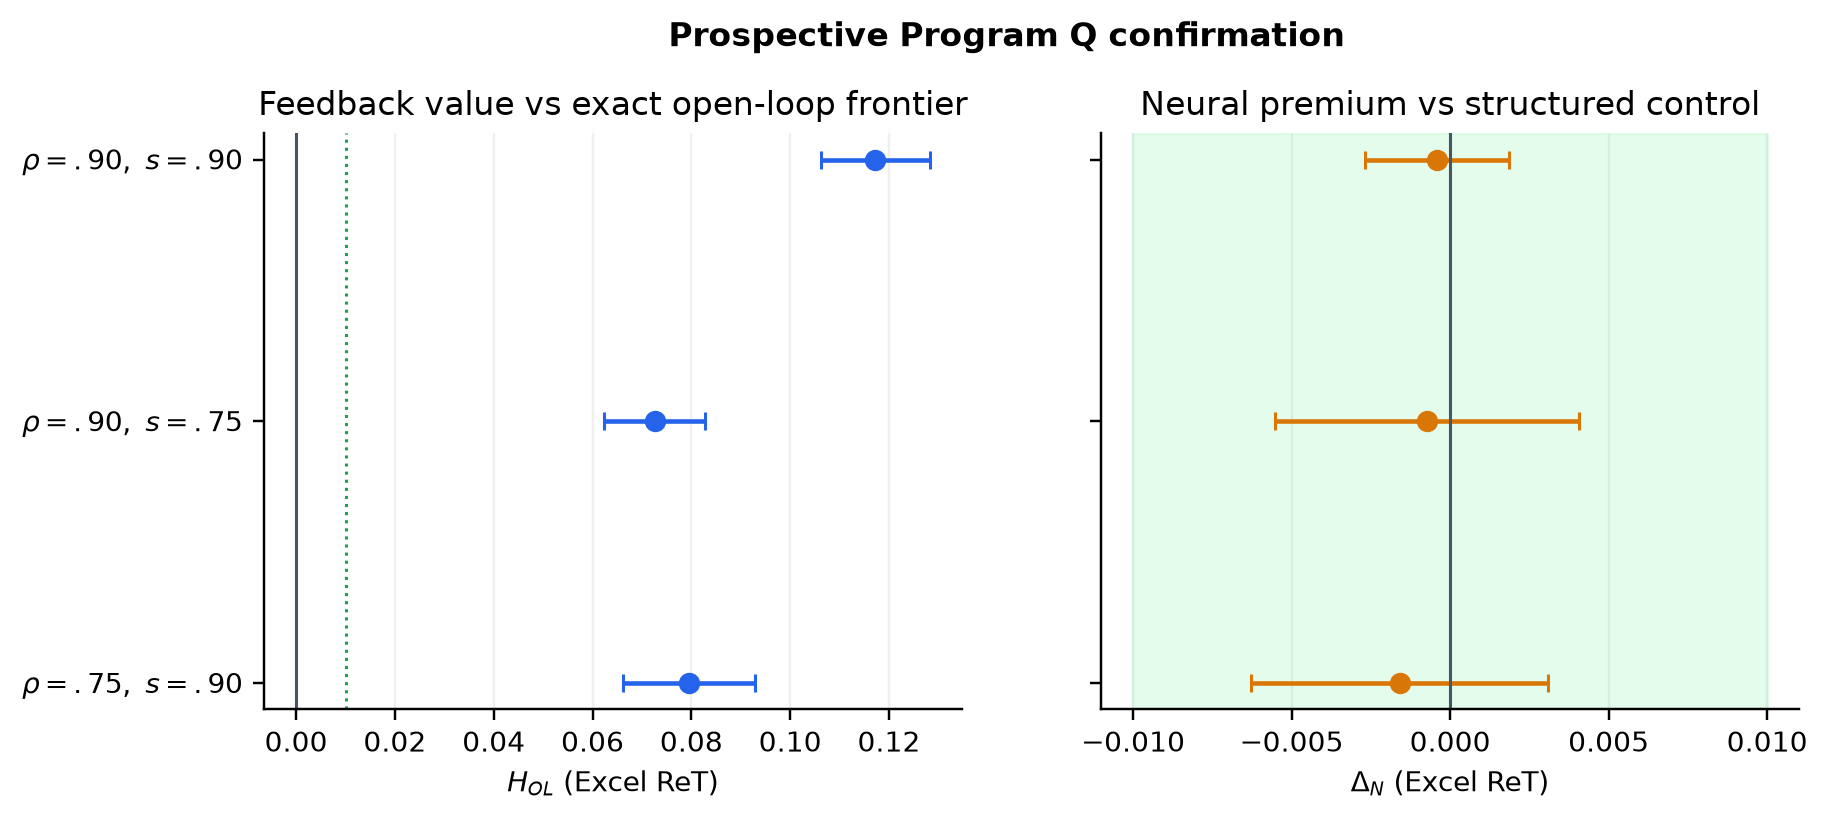
\includegraphics[width=0.92\linewidth]{figure3_feedback_and_neural}
\caption{Simultaneous Program Q confirmation intervals. The learner has substantial feedback value over the exact static frontier (left) and no identified neural premium over structured control (right). The shaded band is the prespecified equivalence region.}
\label{fig:effects}
\end{figure}

\subsection{Service and ledger boundary}

Worst-product-fill point contrasts against structured control are modestly negative, but their simultaneous lower bounds are -0.02266, -0.02566, and -0.02632. Each crosses the frozen -0.02 non-inferiority margin. The compound Program Q contract therefore ends in \path{STOP_Q_NO_REPLICATED_LEARNED_ADAPTATION}, despite passing the ReT superiority and equivalence endpoints. We preserve this binding label and report its decomposition rather than translating it into a generic failure.

No policy contrast creates lost orders, and the scheduled-resource spread is exactly zero. Relative to structured control, however, RecurrentPPO has 0.12--0.28 more unresolved orders on average and a larger service-loss area. These companion endpoints are directionally consistent with the failed worst-product guardrail. By contrast, relative to the static frontier, the learner sharply improves worst-product fill and reduces unresolved orders. The safety conclusion therefore depends on the comparator: feedback repairs a weak static allocation, but the learned controller does not establish non-inferiority to strong structured feedback.

\begin{table}[htbp]
\centering
\small
\caption{Service, ledger, and resource contrasts against structured control.}
\label{tab:guardrails}
\resizebox{\linewidth}{!}{%
\begin{tabular}{lrrrrrr}
\toprule
Cell & Worst fill & LCB95 & Lost & Unresolved & Service AUC & Resource spread \\
\midrule
rho75\_share90 & -0.01036 & -0.02266 & +0.000 & +0.204 & +908251 & 0.0 \\
rho90\_share75 & -0.01573 & -0.02566 & +0.000 & +0.280 & +1164457 & 0.0 \\
rho90\_share90 & -0.00451 & -0.02632 & +0.000 & +0.119 & +476550 & 0.0 \\
\bottomrule
\end{tabular}
}
\vspace{2pt}
\parbox{0.96\linewidth}{\footnotesize Positive service-loss AUC and unresolved-order contrasts indicate worse learner outcomes. Lost-order contrasts and scheduled-resource spread are exactly zero; worst-product non-inferiority was not established.}
\end{table}


\begin{figure}[htbp]
\centering
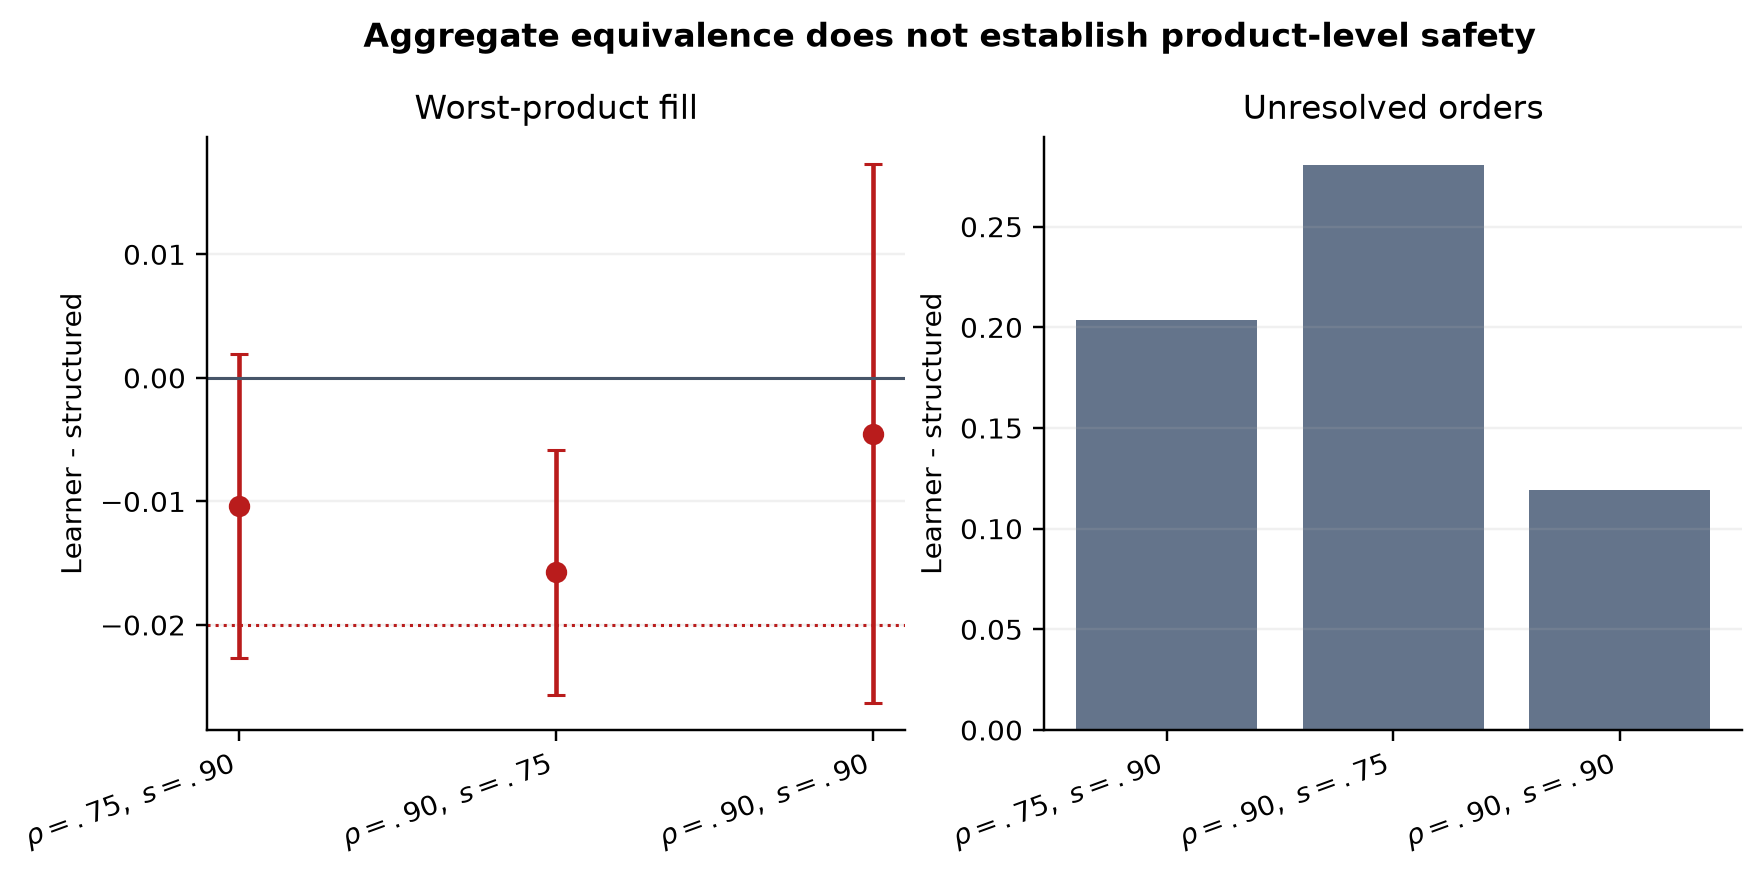
\includegraphics[width=0.88\linewidth]{figure4_service_boundary}
\caption{Service boundary relative to structured control. Error bars for worst-product fill extend to the simultaneous one-sided lower bound. Positive unresolved-order differences are unfavorable.}
\label{fig:service}
\end{figure}

\subsection{Mechanism: feedback rather than calendar discovery}

All trajectory audits pass. Even the least diverse seed-cell combination generates far more than the minimum number of distinct calendars, modal concentration remains low, and at least seven of eight weekly positions vary. Every learner seed beats each of the modal, phase-only, and frequency-matched replacements. This establishes that the observed $\HOL$ is not reproduced by freezing the most common sequence or its marginal action frequency.

The exact static frontier is locally flat near its maximum: in calibration, the first 38 calendars occupy a narrow ReT band. Flatness helps explain why policy-gradient updates need not select a unique rank-one calendar, but it cannot explain away the confirmatory feedback advantage, which is an order of magnitude larger. Instead, the evidence supports a controller-level interpretation: the recurrent learner reacts to causal state and approximates the value already captured by structured feedback.

\begin{table}[htbp]
\centering
\small
\caption{Diagnostics separating feedback from static schedule discovery.}
\label{tab:mechanism}
\resizebox{\linewidth}{!}{%
\begin{tabular}{lrrrrr}
\toprule
Cell & Min unique & Max modal & Min varying & Repl. beaten & Top-38 width \\
\midrule
rho75\_share90 & 125 & 0.082 & 7 & 10/10 & 0.00076 \\
rho90\_share75 & 190 & 0.039 & 7 & 10/10 & 0.00241 \\
rho90\_share90 & 91 & 0.219 & 7 & 10/10 & 0.00807 \\
\bottomrule
\end{tabular}
}
\vspace{2pt}
\parbox{0.96\linewidth}{\footnotesize Replacement denotes the weakest seed count across modal, phase-only, and frequency-matched controls. Top-38 width is descriptive calibration evidence from the exact frontier, not a confirmation estimand.}
\end{table}


\section{Discussion}

\subsection{What the result establishes}

The study establishes robust value of within-campaign feedback. This is stronger than showing that PPO beats several handpicked policies, because every admissible open-loop calendar is evaluated. It is weaker than showing that a neural controller is uniquely capable: the structured controller extracts practically the same ReT with the same deployable information. The appropriate conclusion is therefore ``adaptive feedback without a neural premium.''

This conclusion is useful for industrial modeling. If a structured controller is available, it provides interpretability and explicit feasibility handling. We therefore measured batch-one action-selection latency separately from outcome quality, excluding DES construction and observation replay. On one Apple-silicon system, over 5,000 repetitions on 24 causal observations, median latency was 0.573 ms for RecurrentPPO and 0.082 ms for the reselected structured family. These hardware-specific descriptive measurements identify no computational advantage for the recurrent policy. A neural controller should not be justified by a contrast that only identifies feedback value.

\subsection{Metric semantics and safety}

Exact reproduction of a source formula is necessary but not sufficient for safe optimization. The workbook-visible ReT mean does not contain every unresolved order as a primary row. Replacing it retrospectively would break lineage with the original construct; optimizing it without a complete ledger would allow favorable selection. Our solution is to preserve official ReT as the primary construct while making service and conservation outcomes mandatory companions.

The worst-product result illustrates the need. Aggregate ReT equivalence coexists with an unconfirmed product-level service floor. We do not describe the learned policy as safe or deployment-ready. Future constrained or shielded controllers would constitute new prospective studies; they cannot revise the Program Q adjudication.

\subsection{Relation to Garrido's learning agenda}

Program Q operationalizes the first step in Garrido et al.'s agenda: a DES observation is converted into a decision and returned to the simulation, creating learned closed-loop control \cite{garrido2024iccl}. It does not cure the proposed cross-run ``Alzheimer effect.'' Each Program Q episode resets physical and recurrent state, and the primary environment disables Garrido-native risks. Demonstrating accumulated learning requires a separate retained-versus-reset treatment across campaign sequences, a physical reset, and a structured controller allowed to retain the same information. We reserve that question for Q-R1.

\begin{table}[htbp]
\centering
\small
\caption{Supported and unsupported interpretations.}
\label{tab:claim_boundary}
\begin{tabular}{p{0.26\linewidth}p{0.18\linewidth}p{0.44\linewidth}}
\toprule
Statement & Status & Reason \\
\midrule
Feedback beats the complete static frontier & Supported & Prospective confirmation in all cells with simultaneous positive lower bounds \\
RecurrentPPO has a neural premium & Not supported & Practical equivalence, not superiority, versus structured control \\
The learned policy is deployment-safe & Not supported & Worst-product service margin failed \\
The model learns across campaigns & Not tested here & Program Q resets each episode; Q-R1 is a separate prospective study \\
Results generalize to Garrido-native risks & Not supported & Primary Program Q physics are risk-off and multiproduct researcher-defined \\
The study closes the DES feedback loop & Supported in contract & Actions use causal within-episode observations and beat phase/modal/frequency replacements \\
\bottomrule
\end{tabular}
\end{table}


\section{Limitations}

The first limitation is external validity. The product labels and Markov demand regimes are a disclosed researcher extension. The primary result is risk-off and cannot be generalized to the original disruption taxonomy or to operational military readiness. Second, the finite action space enables an unusually strong exact static benchmark but may compress the residual advantage available over structured control. Third, the learner architecture and hyperparameters were frozen rather than tuned; Program Q therefore evaluates a specified recurrent learner, not the best possible neural architecture. This does not weaken the positive $\HOL$ claim, but it limits universal conclusions about neural methods.

Fourth, the structured family is the strongest tested same-contract family, not a proof of the optimal POMDP policy in the full DES. Our claim is ``best tested structured control,'' not superiority or equivalence to every possible dynamic policy. Fifth, product-level service is not certified. Finally, formula replay with source snapshots does not by itself prove every endogenous same-timestamp ledger convention; the paper therefore states the snapshot semantics and reports the complete audit trail.

\section{Conclusion}

An exact static frontier changes the interpretation of RL performance. RecurrentPPO robustly beats all 65,536 open-loop calendars in a multiproduct supply-chain DES, demonstrating material feedback value. The strongest reselected member of a structured feedback family recovers practically the same value, and the learned policy does not establish worst-product non-inferiority. The resulting contribution is a disciplined separation: feedback can matter greatly even when neural complexity is neither superior nor automatically safe. For simulation studies seeking to integrate AI, exhaustive or appropriately strong structured benchmarks and complete service ledgers are not ancillary checks; they determine what the learning claim means.

\section*{Data and code availability}

The code, frozen contracts, trained checkpoint manifests, confirmation result, direct full-DES audit, and a deterministic table/figure generator are maintained in the public project repository. The full raw confirmation bundle is retained under an immutable checksum manifest; the review branch contains the slim adjudication bundle and a hash-verified compact summary of the exact calibration frontier. A versioned archival DOI will be assigned to the submission release.

\section*{Declaration of competing interest}

The authors declare no known competing financial interests or personal relationships that could have appeared to influence the work reported in this paper.

\section*{CRediT authorship contribution statement}

Authorship identities and role assignments are maintained on the separate title page during anonymous review. The proposed first-author contribution comprises conceptualization, methodology, software, validation, formal analysis, visualization, data curation, reproducibility, and writing of the original draft.

\appendix
\section{Reproducibility boundary}

The manuscript build verifies the SHA-256 digest of the confirmation result, adjudication, independent direct audit, metric audit, learner contract, confirmation contract, and calibration result before producing any table or figure. The compact frontier artifact verifies all 144 source matrices against the frozen raw-file manifest before aggregation. No simulator is rerun during manuscript generation, and no historical verdict is re-adjudicated.

\bibliographystyle{elsarticle-num}
\bibliography{references}

\end{document}
